\documentclass[a4paper,11pt]{article}
\usepackage[ngerman]{babel}
\usepackage[ansinew]{inputenc}
\usepackage{geometry}
\usepackage{graphicx}
\usepackage{ulem}
\usepackage{listings}
\usepackage{color}

\geometry{top=20mm, left=30mm, right=30mm, bottom=20mm}
\parindent 0pt
\lstset{language=SQL} 
\lstset{tabsize=4}
\lstset{showstringspaces=false}


\title{Dokumentation zum Datenbankprojekt}
\author{Katharina Chowanski / Marvin Kleinert / Marius Schidlack}  
\date{\today}

\begin{document}
\maketitle 

\section*{Iteration 1: Modellierung}
\subsection*{1. Entity-Relationship-Modell}
\begin{figure}[htbp]
	\centering
		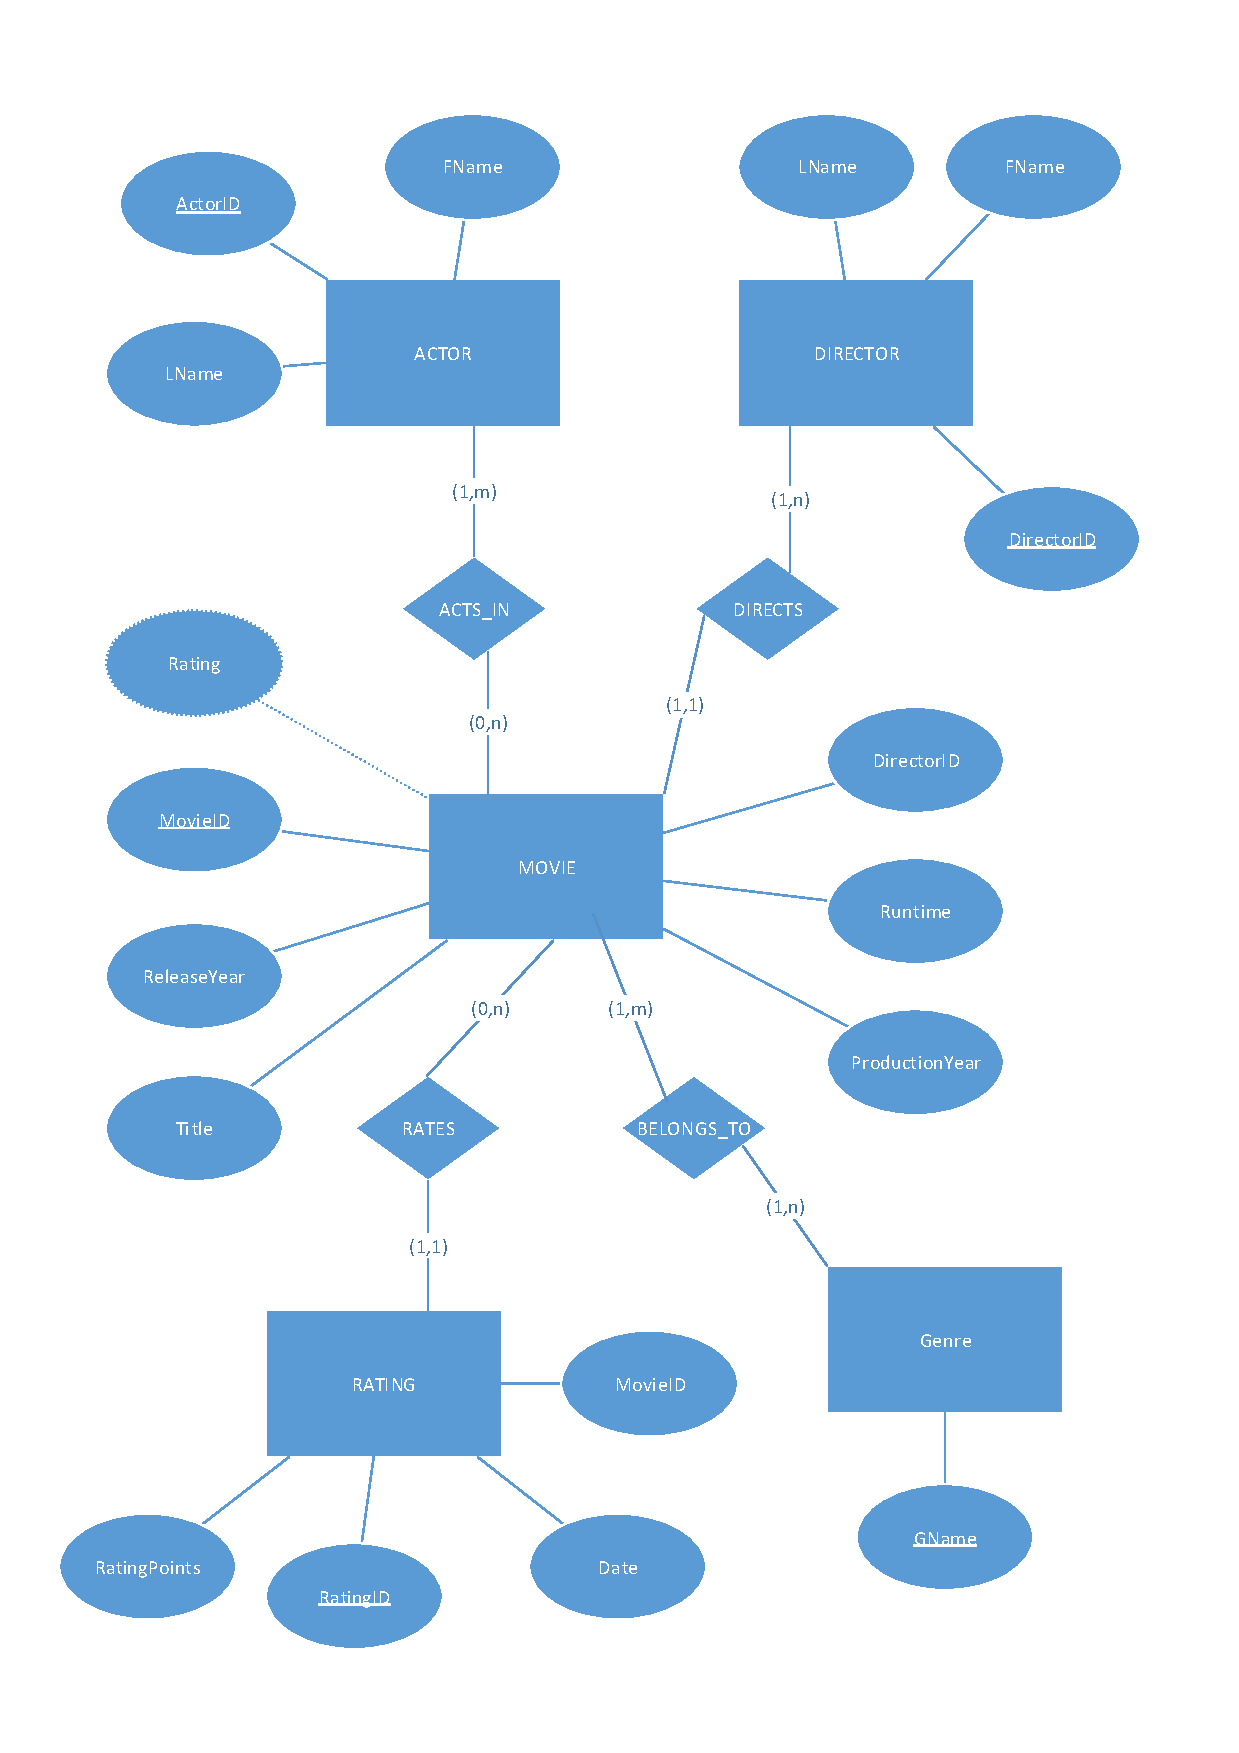
\includegraphics[width=0.85\textwidth]{MoviesER_Portrait.pdf}
	\label{fig:MoviesER}
\end{figure}

\subsection*{2. Relationales Modell}
MOVIE (Title: string; \uline{MovieID}: int; ReleaseYear: int; ProductionYear: int; \\Runtime: int; DirectorID: int; Rating: float)\\[0.5cm]
ACTOR (\uline{ActorID}: int; FName: string; Lname: string)\\[0.5cm]
DIRECTOR (\uline{DirectorID}: int; FName: string; LName: string)\\[0.5cm]
RATING (\uline{RatingID}: int; Date: date; RatingPoints: int; MovieID: int)\\[0.5cm]
GENRE (\uline{GName}: string)\\[0.5cm]
ACTS\_IN (\underline{\dashuline{MovieID}}: int; \underline{\dashuline{ActorID}}: int)\\[0.5cm]
BELONGS\_TO (\underline{\dashuline{GName}}: string; \underline{\dashuline{MovieID}}: int)

\subsection*{3. CREATE-Statements}
\begin{lstlisting}
CREATE TABLE MOVIE 
(Title				varchar(255) NOT NULL,
MovieID				int8 NOT NULL,
ReleaseYear			interval YEAR,
ProductionYear			interval YEAR,
Runtime				int4,
DirectorID			int8 NOT NULL,
Rating				float4,
PRIMARY KEY (MovieID),
FOREIGN KEY (DirectorID) REFERENCES DIRECTOR (DirectorID)
);

CREATE TABLE ACTOR
(ActorID			int8 NOT NULL,
FName				varchar(255),
LName				varchar(255),
PRIMARY KEY (ActorID)
);

CREATE TABLE DIRECTOR
(DirectorID			int8 NOT NULL,
FName				varchar(255),
LName 				varchar(255),
PRIMARY KEY (DirectorID)
);

CREATE TABLE RATING
(RatingID			int8 NOT NULL,
Date				date,
RatingPoints			int4,
MovieID				int8 NOT NULL,
PRIMARY KEY (RatingID),
FOREIGN KEY (MovieID) REFERENCES MOVIE (MovieID)
);

CREATE TABLE GENRE
(GName				varchar(255) NOT NULL,
PRIMARY KEY (GName)
);

CREATE TABLE ACTS_IN
(MovieID			int8 NOT NULL,
ActorID				int8 NOT NULL,
PRIMARY KEY (MovieID, ActorID),
FOREIGN KEY (MovieID) REFERENCES MOVIE(MovieID),
FOREIGN KEY (ActorID) REFERENCES ACTOR (ActorID)
);

CREATE TABLE BELONGS_TO
(GName				varchar(255) NOT NULL,
MovieID				int8 NOT NULL,
PRIMARY KEY (GName, MovieID),
FOREIGN KEY (GName) REFERENCES GENRE (GName),
FOREIGN KEY (MovieID) REFERENCES MOVIE (MovieID)
);
\end{lstlisting}

\section*{Iteration 2: Datentransformation und API}
\subsection*{1. Ver�nderungen im Relationalen Modell}
MOVIE (Title: text; \uline{MovieID}: varchar(9); ReleaseYear: int2; \textcolor{red}{ProductionYear: int2}; \\Runtime: int2; \textcolor{red}{DirectorID: int;} Rating: numeric(3,1), \textcolor{green}{RatingCount: int})\\[0.5cm]
ACTOR (\textcolor{red}{\uline{ActorID}: varchar(9);} \uline{FName: varchar(127)}; \uline{LName: varchar(127)})\\[0.5cm]
DIRECTOR (\textcolor{red}{\uline{DirectorID}: varchar(9);} \uline{FName: varchar(127)}; \uline{LName: varchar(127)})\\[0.5cm]
\textcolor{red}{RATING (\uline{RatingID}: varchar(9); Date: date; RatingPoints: int2; MovieID: varchar(9))}\\[0.5cm]
GENRE (\uline{GName}: varchar(127))\\[0.5cm]
ACTS\_IN (\underline{\dashuline{MovieID}}: varchar(9); \\ \textcolor{green}{\underline{\dashuline{ACTOR.FName}}: varchar(127); \underline{\dashuline{ACTOR.LName}}: varchar(127)})\\[0.5cm]
\textcolor{green}{DIRECTS (\underline{\dashuline{MovieID}}: varchar(9); \underline{\dashuline{DIRECTOR.FName}}: varchar(127); \underline{\dashuline{DIRECTOR.LName}}: varchar(127))}\\[0.5cm]
BELONGS\_TO (\underline{\dashuline{GName}}: varchar(127); \underline{\dashuline{MovieID}}: varchar(9))\\[0.5cm]
Die �nderungen zum urspr�nglichen Relationalen Modell resultieren aus der Sichtung des Datensatzes und bestehen im Wechsel der Prim�rschl�ssel bei den Relationen ACTOR und DIRECTOR von einer in den Daten nicht enthaltenen ID zu Vor- und Nachname, sowie einer neuen Relation DIRECTS. Diese ist n�tig geworden, da in den Daten auch Filme vorkommen, die mehrere Directors haben k�nnen und somit zwischen MOVIE und DIRECTOR eine n:m-Beziehung besteht.

\subsection*{2. Datentransformation mit Java und JDBC}

\subsection*{3. Datentransformation mit SQL}
\begin{lstlisting}[language=SQL]
CREATE TABLE alldata 
	(imdbID			VARCHAR(9), 
	name			TEXT,
	year			INT2, 
	rating			NUMERIC(3,1),
	votes			INT,
	runtime			INT2,
	directors		TEXT, 
	actors			TEXT,
	genres			TEXT);
	
COPY alldata 
FROM 'imdb_top100t_2015-06-18.csv'
FORMAT CSV
DELIMITER '\t';

INSERT INTO movies
(imdbID, title, rel_year, rating, rating_counts, duration)
SELECT imdbID, name, year, rating, votes, runtime
FROM alldata A
WHERE NOT EXSISTS  (SELECT imdbID
					FROM movies	
					WHERE A.imdbID = imdbID);

\end{lstlisting}

Unsere Idee bei der Transformation der Daten ausschlie�lich mit SQL bestand darin, zun�chst eine Tabelle f�r alle Attribute anzulegen, um dann mit der von SQL zur Verf�gung gestellten COPY-Funktion die CSV-Datei mit ihrem Delimiter TAB in die Tabelle zu kopieren. Die gew�nschten Daten f�r die einzelnen Tabellen unserer Datenbank erh�lt man schlie�lich durch Querys auf die neu erzeugte Tabelle.\\[0.5cm]

\subsection*{4. API}
\begin{lstlisting}[language=Java]
public interface DatabaseAPI {
	public String bestMovies (int count);
	public String moviesRating (int from, int to);
	public String moviesRating (int from, int to, int year);
	public String actorsInMovie (String movieTitle);
	public String directorsOfMovie (String movieTitle);
	public String ratingOfMovie (String movieTitle);
	public String genresOfMovie (String movieTitle);
	public String movieInfos (String movieTitle);
	public String moviesOfActor (String fname, String lName);
	public String moviesOfActor 
					(String fname, String lName, int year);
	public String debutOfActor (String fName, String lName);
	public String  moviesOfDirector 
					(String fName, String lName);
	public String  moviesOfDirector 
					(String fName, String lName, int year);
	public String actorsWorkedForDirector 
					(String fName, String lName);
	public String directorWithMostMovies (int year);
\end{lstlisting}
Unsere API orientiert sich an den beispielanfragen in der Projektbeschreibung, umfasst aber zudem noch weitere n�tzliche Anfragen, wie z.B. welche Schauspieler in einem bestimmten Film mitspielen oder wer bei einem bestimmten Fil Regie gef�hrt hat. Exemplarisch folgt nun die Implementierung von zwei Methoden des obigen Interfaces:\\
\begin{lstlisting}[language=Java]
public String actorsInMovie (String movieTitle){
	String sql = 	("SELECT firstname, lastname "
					+ "FROM movies, acts_in "
					+ "WHERE title = ? "
					+ "AND id = movieID ");
	TupleQ[] pstValues = {new TupleQ(1,movieTitle)};
	ResultSet rs = manageQuery (sql, pstValues);
	String retString = resultTable(rs, new TupleR[]
			{new TupleR("firstname",String.class), 
			new TupleR( "lastname", String.class) });	
	return retString;
}

public String debutOfActor (String fName, String lName){
	String sql = 	("SELECT title, rel_year "
					+ "FROM movies, acts_in "
					+ "WHERE firstname = ? "
					+ "AND lastname = ? "
					+ "AND id = movieID "
					+ "AND rel_year > 0 "
					+ "ORDER BY rel_year ASC "
					+ "LIMIT 1 ");
	TupleQ[] pstValues = {new TupleQ(1,fName), 
						new TupleQ(2, lName)};
	ResultSet rs = manageQuery (sql, pstValues);
	String retString = resultTable(rs, new TupleR[]
			{new TupleR("title",String.class),
				new TupleR("rel_year",int.class)});	
	return retString;	
}
\end{lstlisting}

Hauptbestandteil der Methoden bildet die SQL-Abfrage, die zusammen mit den n�tigen Parametern in einer separaten Funktion weiterverarbeitet wird, um sich wederholenden Code zu vermeiden. Dabei werden PreparedStatements verwendet, um m�gliche SQL-Injections durch falsche Eingaben zu verhindern. Auch die Ausgabe der Daten wird in einer separaten Funktion gemanagt, sodass m�gliche �nderungen in der Darstellung f�r die GUI leicht an nur einer Stelle vollzogen werden k�nnen.\\[0.5cm]
 
\section*{Iteration 3: GUI und Datamining}
\subsection*{1. Datamining}


\section*{Auswertung des Projekts}

\end{document}